\chapter{Methodology}

The methodology of this project will be double-faceted, focusing on the development of the simulation itself, and the concurrent audit of
sources used to aide that development.

\section{Simulation Architecture}

The simulation is developed using C++ due to its high performance and stability, and memory management
which will be important for handling large particle counts and their calculations efficiently.

\begin{itemize}
    \item \textbf{Object-orientated design:} Each particle will be considered it's own object. Handling it's own position, radius, and systems such as rendering.
    \item \textbf{Environment:} Development is performed in a Linux environment using the GCC compiler.
\end{itemize}

The simulation also uses Dear ImGui (commonly referred to as \textit{ImGui, imgui, or IMGUI}) to render a Graphical User Interface (GUI), this will provide the user statistics such as the number of particles, performance stats, alongside providing the user the ability to add or remove particles. (\cite{ocornut-imgui})

\section{Approachability Audit}
\subsection{Data Collection Process}

As additions are made to the simulation (e.g the gravitational force), the primary source that was used for that feature will be logged, and its approachability will be scored and logged based on the criteria shown in table \ref{tab:severity}.

\subsection{Evaluation}
At the end of the development of the simulation, the \textbf{Approachability Score \textit{AS}} will be calculated and cross-referenced to the estimated time it had taken to implement the feature the source was used for.

\section{Fundamental Forces}

The first major system we will be implementing are the fundamental forces.

It should be noted that at this point, the project boilerplate has been written, such as the imgui interface, and the ability
to place either a proton \textit{(\proton)}, neutron \textit{(\neutron)}, electron \textit{(\electron)}, 
or photon \textit{(\photon)}, into the sandbox scene.

\begin{figure}[h]
    \centering
    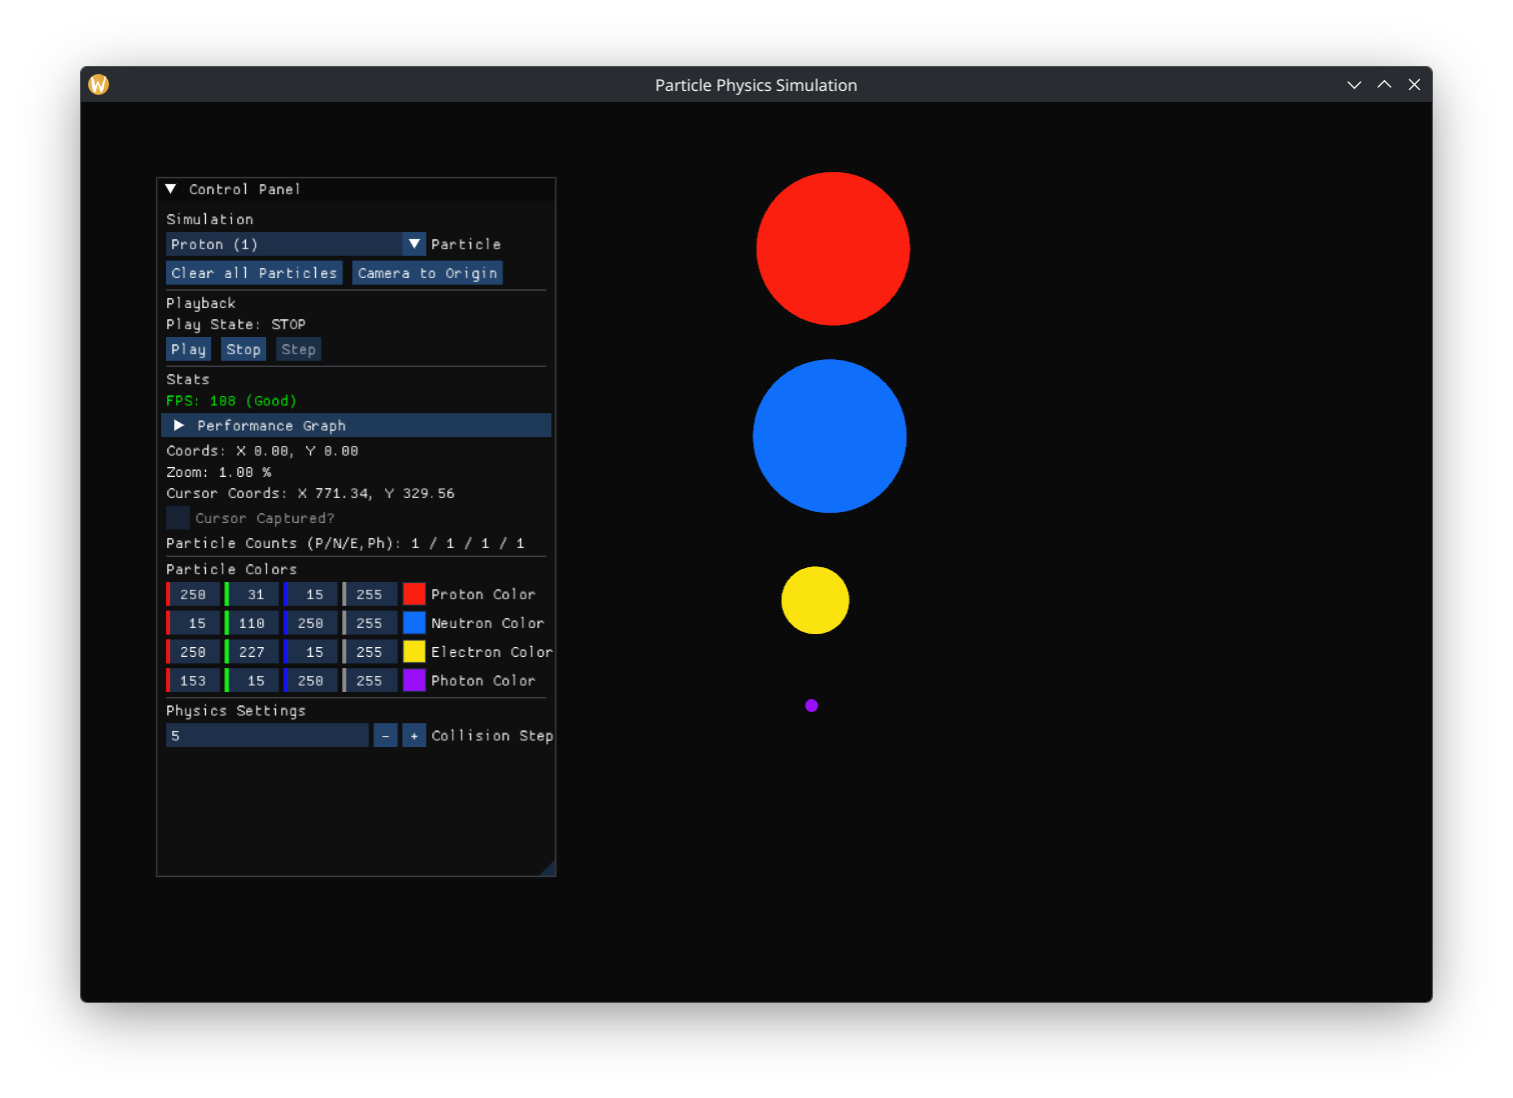
\includegraphics[width=0.8\linewidth]{res/images/initial-project-setup.png}
    \caption{Initial project setup}
    \label{fig:initial-project-setup}
\end{figure}